\documentclass[a4paper,10pt]{article}
\usepackage[utf8]{inputenc}
\usepackage[T1]{fontenc}
\usepackage[italian]{babel}

\usepackage{amsmath}
\usepackage{amsfonts}
\usepackage{amssymb}
\usepackage{graphicx}

\usepackage[left=2cm,right=2cm,top=2cm,bottom=2cm]{geometry}
\geometry{a4paper}

\usepackage{booktabs}
\usepackage{verbatim}
\usepackage{subfig}
\usepackage[italian, sort, noabbrev, capitalise]{cleveref}
\usepackage[bottom]{footmisc}

\usepackage[cdot, thickqspace, squaren]{SIunits}
\usepackage{float}

% macro
\def\code#1{\texttt{#1}}

\title{Esercitazione 11: Semplici circuiti logici e Multivibratori.}
\author{Gruppo BL \\ Candido Alessandro, Luzio Andrea, Mazziotti Fabrizio}

\begin{document}

\maketitle

\section{Scopo e Strumentazione}
Studio dell'applicazione delle porte NAND nella costruzione di semplici circuiti logici e multivibratori.

La strumentazione è quella solitamente presente sul banco di lavoro, e inoltre si è usato:
\begin{itemize}
	\item 2 circuiti integrati \code{SN7400} Quad-NAND Gate;
	\item 1 DIP Switch a 4 interuttori;
	\item 1 diodo \code{1N4148};
	\item 2 diodi LED;
	\item Impulsatore, realizzato nella precedente esperienza;
\end{itemize}

\section{Costruzione di circuiti logici elementari}
Si sono connessi due interruttori tra i due ingressi di una porta NAND, alimentata a $\unit{4.94 \pm 0.03}{\volt}$, e massa e si è posto un diodo LED, con una resistenza di protezione di $\sim \unit{330}{\ohm}$, all'uscita della porta.
Si è verificata la tabella di verità del NAND provando tutte le combinazioni delle posizioni dei due interruttori, verificando lo stato dell'uscita mediante l'accensione del LED.

Si è applicato lo stesso metodo anche gli altri circuiti descritti in questa sezione, e si è verificata la tabella di verità nei vari casi.
Inoltre si è usato l'impulsatore per visualizzare il risultato sull'oscilloscopio; si riportano i grafici nelle \cref{fig:AND,fig:OR,fig:XOR,fig:ADDER}.

\paragraph{AND} Si è realizzato il circuito AND con 2 porte NAND.

\begin{figure}[H]
	\centering
	\begin{minipage}{0.49\textwidth}
		\centering
		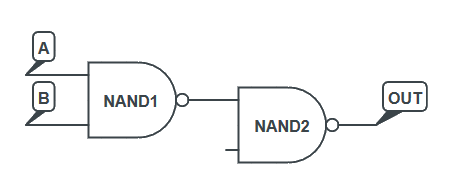
\includegraphics[width=\textwidth]{../grafici/AND1.png}
	\end{minipage}
	\begin{minipage}{0.49\textwidth}
		\centering
		\includegraphics[width=\textwidth]{../grafici/ANDard.pdf}
	\end{minipage}
	\caption{Schema del circuito AND e visualizzazione segnali in I/O}
	\label{fig:AND}
\end{figure}

\paragraph{OR} Si è realizzato il circuito OR con 3 porte NAND.

\begin{figure}[H]
	\centering
	\begin{minipage}{0.49\textwidth}
		\centering
		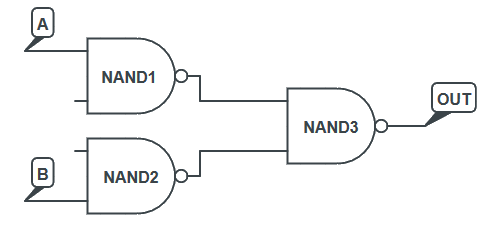
\includegraphics[width=\textwidth]{../grafici/OR1.png}
	\end{minipage}
	\begin{minipage}{0.49\textwidth}
		\centering
		\includegraphics[width=\textwidth]{../grafici/ORard.pdf}
	\end{minipage}
	\caption{Schema del circuito OR e visualizzazione segnali in I/O}
	\label{fig:OR}
\end{figure}

\paragraph{XOR} Si è realizzato il circuito XOR con 4 porte NAND.

\begin{figure}[H]
	\centering
	\begin{minipage}{0.49\textwidth}
		\centering
		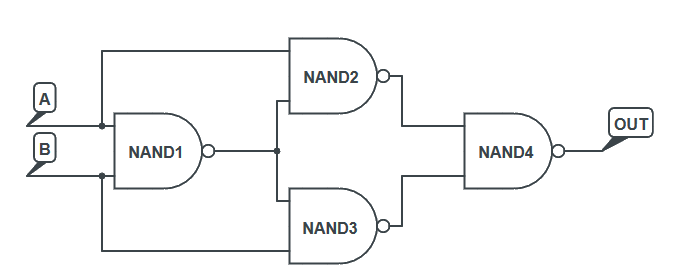
\includegraphics[width=\textwidth]{../grafici/XOR1.png}
	\end{minipage}
	\begin{minipage}{0.49\textwidth}
		\centering
		\includegraphics[width=\textwidth]{../grafici/XORard.pdf}
	\end{minipage}
	\caption{Schema del circuito XOR e visualizzazione segnali in I/O}
	\label{fig:XOR}
\end{figure}


\paragraph{Sommatore ad un bit} Si è realizzato il sommatore ad un bit con 5 porte NAND.

\begin{figure}[H]
	\centering
	\begin{minipage}{0.49\textwidth}
		\centering
		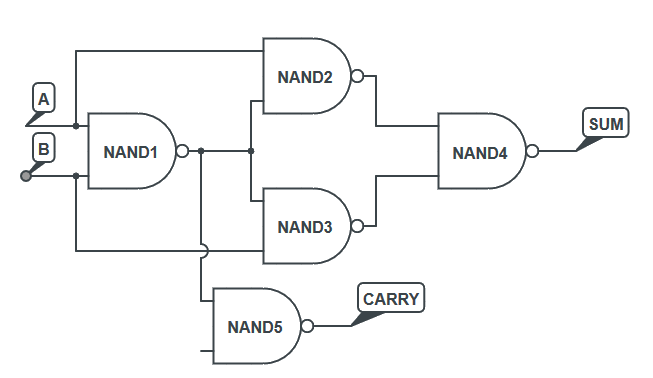
\includegraphics[width=\textwidth]{../grafici/Sommatore1.png}
	\end{minipage}
	\begin{minipage}{0.49\textwidth}
		\centering
		\includegraphics[width=\textwidth]{../grafici/ADDERard.pdf}
	\end{minipage}
	\caption{Schema del sommatore ad un bit e visualizzazione segnali in I/O}
	\label{fig:ADDER}
\end{figure}

\subsection{Osservazione} Negli schemi elettrici mostrati nelle \cref{fig:AND,fig:OR,fig:XOR,fig:ADDER} si può notare che per alcune porte NAND si è lasciato un ingresso flottante, quando si voleva usarle come porte NOT. Si è sfruttato infatti il fatto che gli ingressi flottanti delle porte corrispondono ad un valore \code{HIGH}, secondo la logica TTL.
Tenendo conto di questo si ottiene infatti (\code{HIGH-HIGH} $\rightarrow$ \code{LOW}) e (\code{LOW-HIGH} $\rightarrow$ \code{HIGH}), cioè il comportamento richiesto per una porta NOT.

Si sarebbe potuto connettere gli ingressi insieme, così da avere in uscita ancora una volta un NOT, infatti (\code{HIGH-HIGH} $\rightarrow$ \code{LOW}) e (\code{LOW-LOW} $\rightarrow$ \code{HIGH}) secondo la tabella di verità di una porta NAND, ed essere indipendenti dalla logica usata; si è preferito fare così solo per risparmiare qualche connessione sulla basetta e avere un po' più di ordine (fisico, e quindi anche concettuale).

Si è applicato lo stesso metodo anche nei circuito successivi, anche se gli schemi dei circuiti mostrano gli input connessi insieme perché tratti dalla scheda (vedi \cref{fig:MONO,fig:AST,fig:SQGEN}).

\section{Multivibratore MONOSTABILE}

\begin{figure}[H]
	\centering
	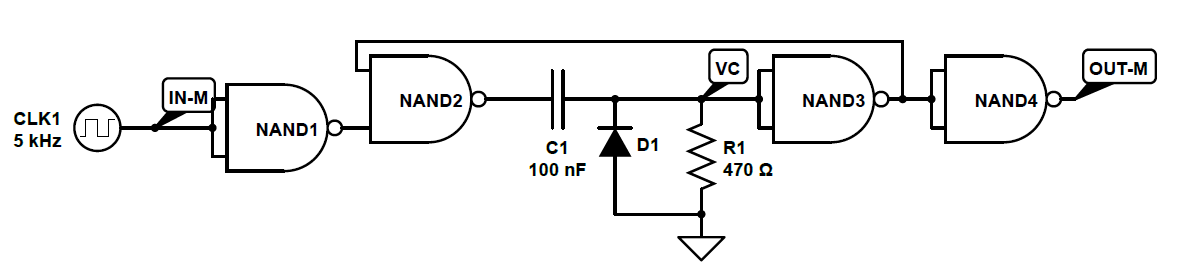
\includegraphics[width=0.9\textwidth]{../grafici/Monostabile.png}
	\caption{Schema del circuito del multivibratore monostabile}
	\label{fig:MONO}
\end{figure}

\section{Multivibratore ASTABILE}

Si è montato il circuito in \cref{fig:AST}.

\begin{figure}[H]
	\centering
	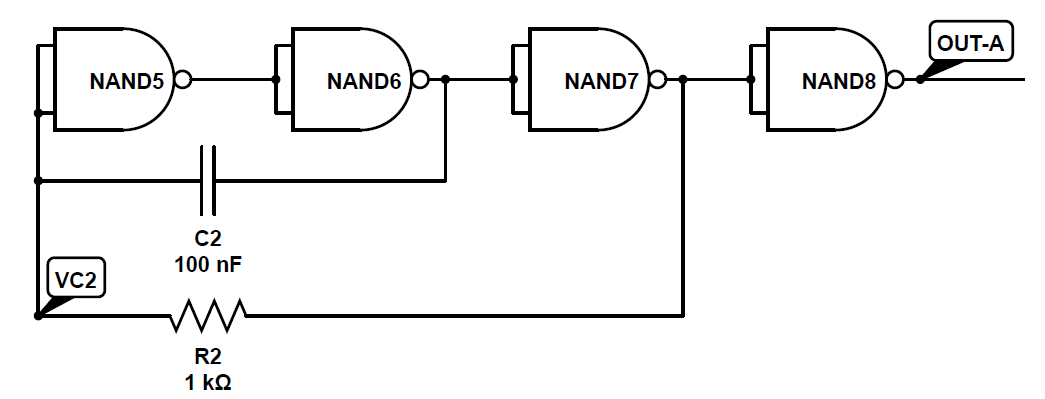
\includegraphics[width=0.7\textwidth]{../grafici/Astabile.png}
	\caption{Schema del circuito del multivibratore astabile}
	\label{fig:AST}
\end{figure}

I componenti impiegati sono stati misurati con il tester digitale, e sono:

\begin{table}[H]
	\centering
	\begin{tabular}{cc}
		$R_2 = \unit{990 \pm 10}{\ohm}$ & $C_2 = \unit{109 \pm 5}{\nano\farad}$\\
	\end{tabular}
\end{table}

Si è verificato che in uscita, OUT-A, la forma d'onda fosse un'onda quadra; si sono misurati il periodo, $\Delta T$, e il duty-cycle, $\delta$, dell'onda, ottenendo:

\begin{table}[H]
	\centering
	\begin{tabular}{cc}
		$\Delta T = \unit{210 \pm 1}{\micro\second}$ & $\delta = \unit{72.0 \pm 4}{\micro\second}$\\
	\end{tabular}
\end{table}

Si riporta quindi la forma d'onda su OUT-A (azzurra) in \cref{fig:ASTosc}, assieme alla forma d'onda presente su VC$2$ (gialla).

\begin{figure}[H]
	\centering
	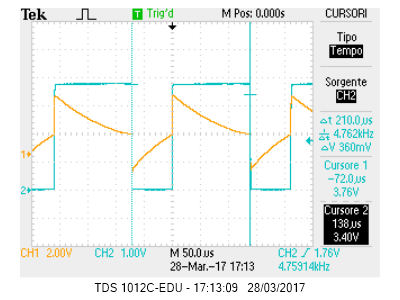
\includegraphics[width=0.7\textwidth]{../grafici/astabileOSC.png}
	\caption{Schema del circuito del multivibratore astabile}
	\label{fig:ASTosc}
\end{figure}

La forma d'onda presente su VC$2$ è il risultato delle curve esponenziali di carica e scarica del condensatore (in realtà sono sempre cariche, perché non si scarica mai liberamente senza una tensione esterna ai capi).

\paragraph{Interpretazione} Per spiegare il comportamento del circuito si deve considerare che la porta NAND$7$ forza la sua uscita ad assumere un valore che sia ben definito, come \code{HIGH} o come \code{LOW}, e altrettanto fa la porta NAND$6$: in questo modo il ramo $R_2-C_2$ ha sempre una differenza di potenziale approssimativamente fissata ai suoi capi, di cui l'unica cosa che varia sostanzialmente è il segno.

Il condensatore si carica dunque, modificando in modo continuo il valore di tensione sul NAND$5$, e raggiunta una data soglia (che risulta essere la stessa in salita in discesa, vedi \cref{fig:ASTosc}), fa commutare NAND5, che a cascata porta tutti gli altri NAND a commutare (sono collegati a catena, l'input di uno all'output del precedente, vedi \cref{fig:AST}).

Il tempo di carica del condensatore è determinato dai valori di $R_2$ e $C_2$, e dalla soglia a cui commuta NAND$5$\footnote{per tempi troppo brevi diventano rilevanti i ritardi delle porte, ma a quel punto non è più possibile considerare come simultanea la commutazione complessiva descritta prima e il circuito può smettere di comportarsi come atteso nel caso descritto}.

Si nota inoltre che all'istante in cui tutte le porte NAND commutano, anche la tensione su VC$2$ salta: infatti il condensatore, che non ha il tempo di scaricarsi, genera la stessa differenza di potenziale tra l'output del NAND$6$ e l'input del NAND$5$ (cioè VC$2$) che generava prima della commutazione, cambiando però istantaneamente il valore dell'output del NAND$6$ cambia pure istantaneamente il valore di VC$2$.

\subsection{Linearità del periodo}
Si è quindi verificato che l'andamento del periodo in funzione della resistenza $R_2$ fosse lineare, come atteso: infatti l'andamento del tempo caratteristico del ramo $R_2-C_2$ è lineare nel valore di $R_2$, ed il periodo è determinato linearmente da tale tempo caratteristico (se il condensatore impiega il doppio del tempo per raggiungere la soglia il periodo sarà doppio).

Si sono provati altri $4$ valori per la resistenza $R_2$, oltre a quello impiegato già precedentemente, e si è eseguito un fit lineare con tutti e $5$ i valori. Si riportano dunque il grafico del fit e la tabella con le misure, rispettivamente \cref{fig:ASTfit,tab:ASTfit}.

\begin{figure}[H]
	\centering
	\begin{minipage}{0.49\textwidth}
		\centering
		\includegraphics[width=\textwidth]{../grafici/FITastabile.pdf}
		\caption{}
		\label{fig:ASTfit}
	\end{minipage}
	\begin{minipage}{0.49\textwidth}
		\centering
		\resizebox{0.7\textwidth}{!}{
			\input{../tabelle/tab_astabileRes.txt}}
		\captionof{table}{}
		\label{tab:ASTfit}
	\end{minipage}
\end{figure}

Si verifica che la linearità è ottima, e si riportano di seguito i parametri di fit:

\begin{table}[H]
	\centering
	\begin{tabular}{cccc}
		$\chi^2/ndof = 1.60/3$ & $m = \unit{196 \pm 4}{\micro\second / \kilo\ohm}$ & $q = \unit{16 \pm 4}{\micro\second}$ & $corr_{mq} = -0.97$\\
	\end{tabular}
\end{table}

Dove si è indicato con $m$ il coefficiente angolare, con $q$ l'intercetta e con $corr_{mq}$ il coefficiente di correlazione, che risulta prossimo a ~$-1$ come atteso per una retta.

\section{Generatore di onda quadra}

\begin{figure}[H]
	\centering
	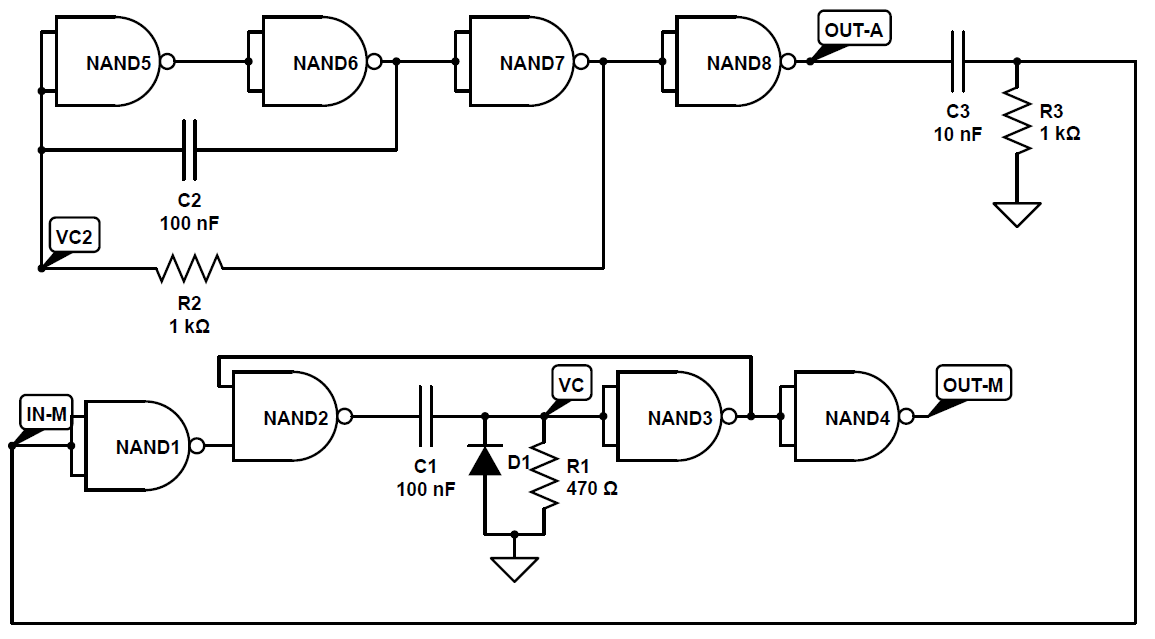
\includegraphics[width=0.8\textwidth]{../grafici/SqGen.png}
	\caption{Schema del circuito del generatore di onda quadra}
	\label{fig:SQGEN}
\end{figure}


\end{document}